\documentclass[fleqn,xcolor={usenames,dvipsnames},notes,aspectratio=169]{beamer} % [notes=only]
\usepackage{amsmath} % {amssymb,amsfonts}

\usepackage{ulem}

% \usepackage{array,adjustbox} % url
% \usepackage{pifont,marvosym} % \ding

% \usepackage{multimedia}
% \usepackage[normalem]{ulem}
% \usepackage{framed,color,ragged2e}
% \usepackage[absolute,overlay]{textpos}
% \definecolor{shadecolor}{rgb}{0.8,0.8,0.8}

\usetheme{boxes}
\setbeamertemplate{navigation symbols}{}
\usepackage{xcolor}
\usepackage{tikz}
\usetikzlibrary{shapes,arrows}
\usetikzlibrary{tikzmark,positioning}
\usetikzlibrary{calc}
\usepackage{tikz-cd}

\newtheorem*{rawnamedtheorem}{\therawnamedtheorem}
\newcommand{\therawnamedtheorem}{\error}
\newenvironment{namedtheorem}[1]{\renewcommand{\therawnamedtheorem}{#1}
   \begin{rawnamedtheorem}}
  {\end{rawnamedtheorem}}


\title{Cryptographic goals beyond key exchange and signatures}
% \subtitle{Cryptography for decentralization}

\author[Jeff Burdges]{Jeff Burdges}
\institute{
  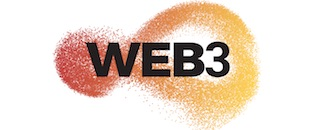
\includegraphics[scale=0.25]{logos/web3logo.jpg}. % web 3 foundation
  \hspace*{5pt}
  \includegraphics[scale=0.15]{logos/gnunet-logo.pdf}
}
\date{27.12.2017}

\begin{document}

{\setbeamertemplate{footline}{}
\begin{frame}
\titlepage
\end{frame}
}
% \note{Hello, happy to be here, etc.}
\setcounter{framenumber}{0}

% \begin{frame}
% \titlepage
% \end{frame}


\begin{frame}
Not about zero-knowledge proofs
\end{frame}


\begin{frame}{Part I:  Mix networks}
\begin{center}
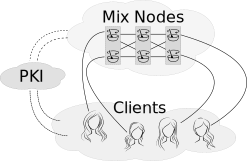
\includegraphics[width=0.8\textwidth]{pics/mix/initial}
\end{center}
\end{frame}


\begin{frame} 
A mix network packet is a header $(\alpha,\beta,\gamma,\ldots)$ and a body $\delta$.

\bigskip

\def\svgwidth{\columnwidth}
\input{pics/mix/sphinx.pdf_tex}

\end{frame}


\begin{frame}[t]{Single-use Reply Blocks (SURBs)}
% We've bi-directional messaging {\it if} both parties know one another.. \\ \smallskip
% \hspace*{5pt} but what if they cannot know one another?

Anonymous receivers matter: \\
\hspace*{10pt} Journalistic sources \\
\hspace*{10pt} Services: CENO, money, etc. \\
\hspace*{10pt} Protocol ACKs!

\bigskip

\def\svgwidth{\columnwidth}
\input{pics/mix/surb.pdf_tex}

\end{frame}


\begin{frame}{Network overhead}

\begin{align*}
\mathrm{SURB} &\approx 5\,\mathrm{hops} * (\mathrm{pk} + 16\,\mathrm{nodeid} + 16\,\mathrm{MAC} + 1) \\
\mathrm{packet} &\approx 2 * \mathrm{SURB} + \mathrm{body} \\
\mathrm{traffic} &\approx 2 * (5\,\mathrm{hops} + 1) * 20\,\mathrm{cover} * \mathrm{packet} \\
\mathrm{maintenance} &\approx 20\,\mathrm{usage} * (5\,\mathrm{hops} + 1) *  \mathrm{SURB} \\
\mathrm{overhead} &= \mathrm{traffic} + \mathrm{maintenance} \\
 &\approx 3000 * \mathrm{pk} + \cdots \quad\textrm{per real message}
\end{align*}

\bigskip\pause

{\bf Idea:}  Keep $\mathrm{pk}$ small and reuse it..

\begin{align*}
\mathrm{SURB} \approx \mathrm{pk} + 5\,\mathrm{hops} * (16\, \mathrm{nodeid} + 16\,\mathrm{MAC} + 1) 
\end{align*}

\end{frame}


\begin{frame}{Sphinx packet format}
A Sphinx header is a tuple $(\alpha,\beta,\gamma)$ where \\

 \vspace*{-18pt} \[
\left. \begin{array}{@{}rl@{}}
  \alpha & \text{is an elliptic curve point,}\\
  \beta & \text{is routing data onion encrypted with a stream cipher,}\\
  \gamma & \text{is a MAC for $\beta$, and} \\
\end{array} \right\} \text{header}
\]  % https://tex.stackexchange.com/questions/240868/how-to-write-cases-with-latex

\def\svgwidth{\columnwidth}
\input{pics/mix/sphinx-kex.pdf_tex}

\end{frame}


\begin{frame}[t]{Sphinx packet format}
Aim: Post-quantum key exchanges with
\begin{itemize}
\item long-term keys, 
\item a blinding operation, 
\item that hybridises with ECDH,
\item and not too bespoke.
\end{itemize}

% \\ \hspace*{10pt} the public and private keys?

\bigskip
\only<1>{
In LWE, a space efficient blinding operation
\begin{itemize}
\item requires FHE bootstrapping,
\item which makes things bespoke, and
\item hybridising with ECDH sounds impossible.
% \item long term keys are not prioritised 
\end{itemize}

\bigskip
We could adapt SIDH with a blinding operation, but highly bespoke and \\
hybridising with ECDH remains impossible, due to sending basis.
}
\only<2>{No Fujisaki-Okamoto transform!}
\end{frame}


\begin{frame}[t]
CSIDH provides a provides a {\it general purpose} post-quantum key exchange \\
with {\it long-term keys} and a {\it blinding operation}.

\bigskip

Can CSIDH hybridise with ECDH?  \pause Yes: 

\medskip

Ward Beullens, Thorsten Kleinjung, and Frederik Vercauteren \\
{\it CSI-FiSh: Efficient Isogeny based Signatures through Class Group Computations}.  \url{https://eprint.iacr.org/2019/498}

\bigskip\bigskip\pause
{\bf Question:}  Batch key exchange perhaps?

\end{frame}


\begin{frame}{Mix network PKI: Too many public keys!}

\sout{Identity} Index-based encryption DKG:
$i$th node ``broadcasts''
\begin{itemize}
\item their public key $A_i = a_i G_1$, 
\item a proof of possession, and
\item the IBE secret keys $a_i H_2(j)$ for $j \neq i$.
\end{itemize}
If some magical MPC enforces this, then we have
\begin{itemize}
\item everyone knows a network public key $A = \sum_i A_i = (\sum_i a_i) G_1$, and
\item the $j$th node knows their IBE secret key $S_j = (\sum_i a_i) H_2(j)$.
\end{itemize}
A key exchange with the $j$th node is given by
$$ e(u A,H(j)) = e(u G_1,S_j) $$

\medskip

{\bf Question:}  Any ideas for isogenies based IBE + DKG?

\end{frame}


\begin{frame}{Part II:  Consensus}

Not discussing batch and aggregate verification

\bigskip
\hspace{20pt}Instead discuss shared randomness

\end{frame}


\begin{frame}[t]{Verifiable Random Functions (VRFs)}

VRF is a PRF keyed by a secret key and verifiable using a public key, \\
often also signature scheme ala RSA-FDH, BLS, hash-based, etc.

\begin{align*}
\mathrm{VRFSign}_{\mathrm{sk}} &: x \mapsto (y,\pi) \\
\mathrm{VRFVerify}_{\mathrm{pk}} &: (x,y,\pi) \mapsto \{0,1\} 
\end{align*}

\medskip

Input $x$ must be collaboratively generated after the public key!  (Ouroboros Praos)

\medskip

Applications often require only that some $x$ work.

\bigskip
\bigskip

{\bf Question:}  Isogenies VRF?

\end{frame}


\def\seed{x} % {\mathtt{seed}}

\begin{frame}[t]{Verifiable Delay Functions (VDFs)}
\vspace{-20pt}
\begin{align*}
\mathrm{VRFProve} &: \seed \mapsto (y,\pi) \\
\mathrm{VRFVerify} &: (\seed,y,\pi) \mapsto \{0,1\} 
\end{align*}

\medskip

Assumes some bound on $T_O/T_S$ where
\begin{itemize}
\item $T_O$ is the running time of public, readily available, and inexpensive implementations of $\mathrm{VRFProve}$, and \\
\item $T_S$ is the running time of secret or proprietary implementations of $x \mapsto y$.
\end{itemize}

\bigskip

Almost all applications mirror applications of threshold cryptography. \\ \medskip

If $\seed = H(\seed_1 || \ldots)$ then any $\seed_i$ released less than $T_S$ before start believes $y$ is random. 

\bigskip\bigskip

Important part is making $\seed \mapsto y$ be ``highly sequential''.

\end{frame}


\begin{frame}[t]
 
Let $e_Z : Z_1 \times Z_2 \to T$ be a pairing on elliptic curves $Z \in \{ X, Y \}$ \\ \smallskip
with slooow dual isogenies $\phi : Y \to X$ and $\phi^* : X \to Y$. \\

\bigskip
$$ 
\underbrace{
 e_Y \bigl( H_1(\seed), \overbrace{\phi G_2}^{const} \bigr)
=
 e_X \bigl( \overbrace{\phi^* H_1(\seed)}^{VDFProve}, G_2 \bigr)
}_{VDFVerify}
$$

\bigskip
\bigskip

Luca De Feo, Simon Masson, Christophe Petit, and Antonio Sanso. \\
{\it Verifiable Delay Functions from Supersingular Isogenies and Pairings}.
\url{https://eprint.iacr.org/2019/166}

\end{frame}


\begin{frame}[t]{Parallel time-lock puzzles}
\vspace{-20pt}
\begin{align*}
\mathrm{VRFEncrypt}_x &: \mathtt{msg} \mapsto \bigl( U,E_s(\mathtt{msg}) \bigr) 
\quad\textrm{after $\seed$ but before $T_S$} \\
\mathrm{VRFDecrypt}_y &: \bigl( U,E_s(\mathtt{msg}) \bigr) \mapsto \mathtt{msg}
\quad\textrm{after $T_O$}
\end{align*}

% \medskip

% Anyone computes $U = u G_2$ and sends ciphertexts $\bigl( U,E_s(\mathtt{vote}) \bigr)$,  \\
% \hspace*{3pt} with $T_S$ after $\seed$ revealed. % but well before $\phi^* H_1(\seed)$.

$$
 e_Y \bigl( H_1(\seed), \overbrace{\phi G_2}^{const} \bigr)^u 
= s =
 e_X \bigl( \overbrace{\phi^* H_1(\seed)}^{VDFProve}, \underbrace{u G_2}_{U} \bigr) 
$$ 

\bigskip
\bigskip

Applications:  Auctions, Voting, ...

\end{frame}


\end{document}
\endinput



% \begin{frame}
% \end{frame}





\begin{frame}[fragile]{Sphinx packet format}
Aim: post-quantum key exchanges support with blinding operation for both the public and private keys?

\begin{tikzcd}
L \arrow[dd, "\forall \delta"'] \arrow[rr, "\varepsilon"] &  & U(L) \arrow[lldd, "\exists ! f"] \\
 &  &  \\
D &  & 
\end{tikzcd}
\end{frame}



% {\it SeaSign: Compact isogeny signatures from class group actions} \\
% by Luca De Feo and Steven D. Galbraith.  \url{https://eprint.iacr.org/2018/824}

